\chapter[Compositional exploration of fluid subspaces]{Compositional explorations of fluid subspaces}
\label{chap:chap6}

With our sonification system from Chapter \ref{chap:chap5} in hand, we now delve into its implications for composition. The process of musical composition, at its core, focuses on different
organizations of time. Commonly, we organize our thoughts and experiments on different timescales: the microlevel, which governs very short durations such as individual notes
or even samples, the mesolevel, which is an intermediate scale which governs larger groups such as phrases or themes, and the macrolevel, which governs the overall form and structure of a piece of music. 

\section{Mode Isolation}
The simplest compositional parameter of interest is the activation or deactivation of individual modes. While a physically accurate subspace re-simulation will in general, at each time step, require a linear combination of each of the $r = 150$ modes, it is also possible to evolve the velocity fields over time according to algorithmic rules rather than physics-based rules. We imagine the $r$ modes as a sort of configuration space, so that a corresponding set of $r$ weights maps to a particular spatial and aural phenomenon. As such, the most elementary experiment is the sequential activation of one mode at a time, creating a corresponding fluid shape of `vibration' which is mapped to its related ``frequency'' according to the system explained in Chapter 5. A low-,\footnote{Low: \url{https://www.youtube.com/watch?v=CAoQLYr8doE}}  medium-,\footnote{Medium: \url{https://www.youtube.com/watch?v=Vwpi6U7AD5A}} and high-frequency mode\footnote{High: \url{https://www.youtube.com/watch?v=o0UtONgtpFo}} are each shown isolated in the referenced videos. 

Because each mode in isolation can be regarded as a musical note, this strategy allows us to carry out musical composition on the note level, producing simple melodies. Without a principled way to choose a rhythm,
however, we are left only to general aesthetic considerations. An example of such a mode-based melody \footnote{Melody: \url{https://www.youtube.com/watch?v=N6fzJXbn2ts}} is demonstrated in the referenced video.

\section{Mode Superposition}
The next experiment to try is the superposition of modes, creating mixtures of the modal vibration shapes in the spatial domain and harmonies in the audio domain. Again, the physics-based time evolution governs a complex coupling of the modal weights that resists simple exploration, so we turn to simple algorithmic rules to better understand the system. We can see the result of mixing a low-, medium-, and high-frequency mode with equal proportions.

\begin{figure}
	\centering
	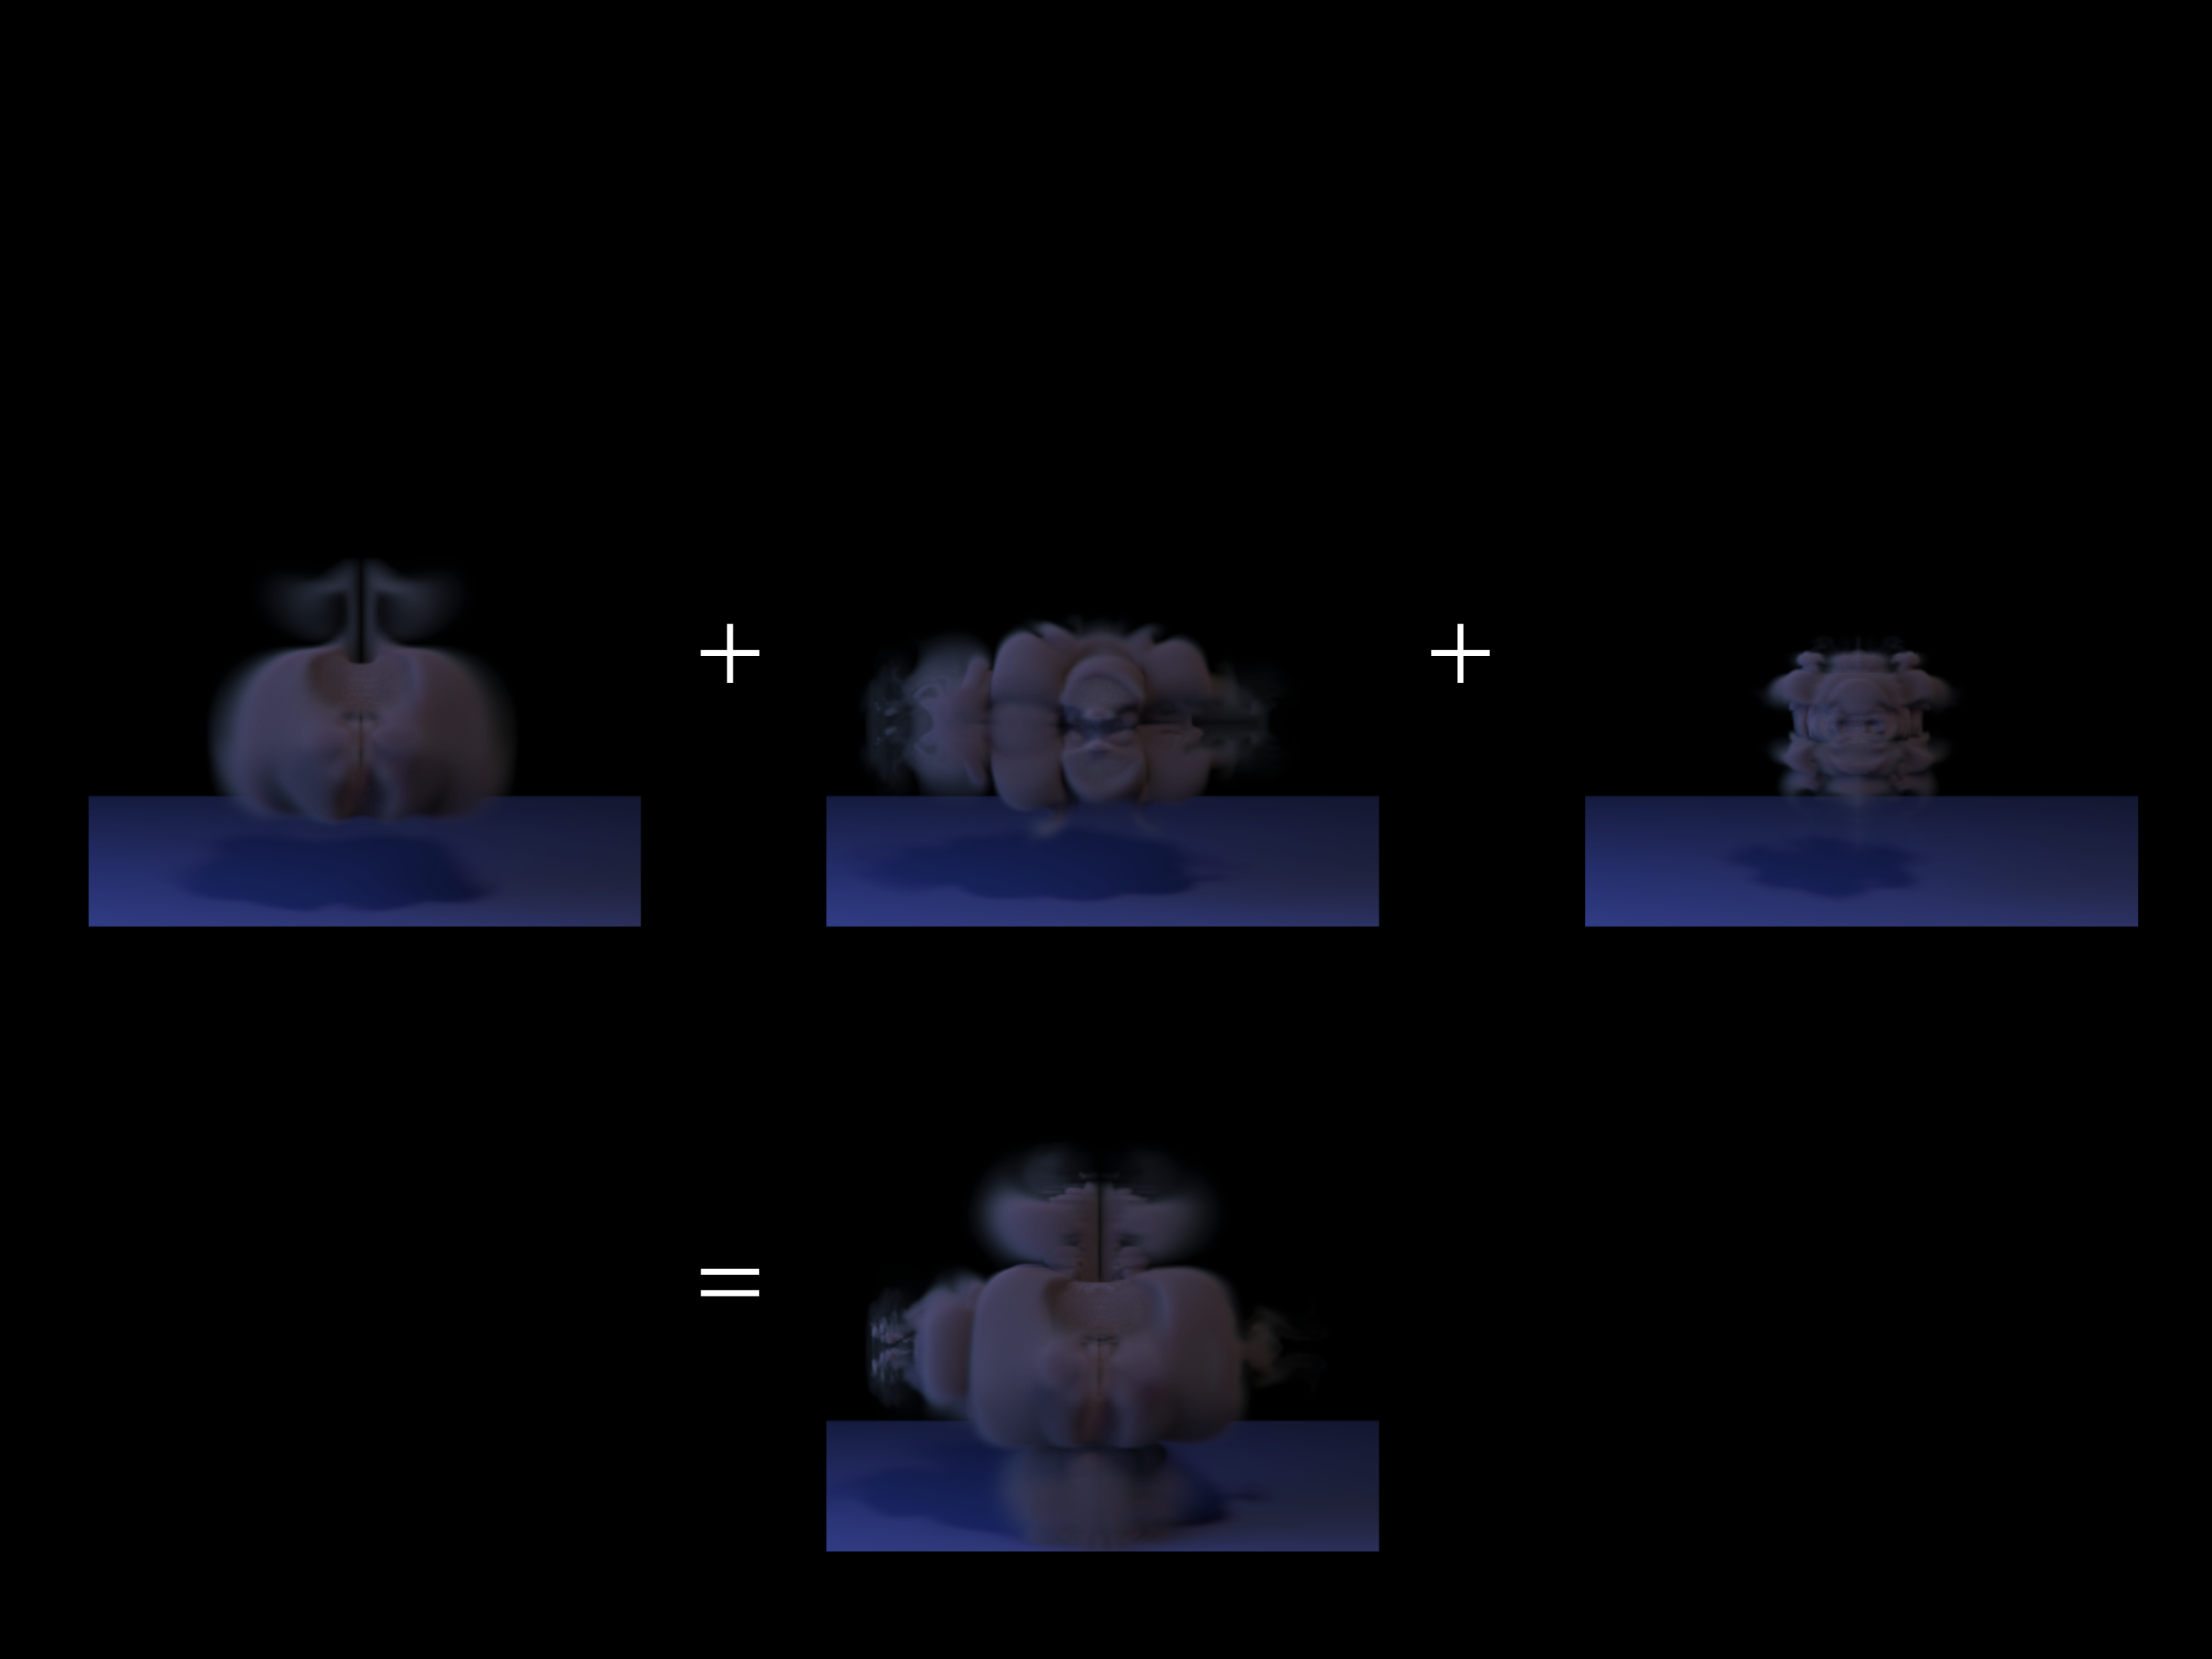
\includegraphics[width=\textwidth]{chap6/figures/superposition.png}
	\caption{\em Three individual modes in superposition produce a mixed modal shape.}
\label{fig:superposition}
\end{figure}

\section{Dynamic Control}
If we define the {\em energy} of a fluid snapshot in time as the $L_2$ norm of the vector of modal weights, then we see that as time unfolds, the energy waxes and wanes according to the strength
of the various modal weights. Accordingly, the sound increases or decreases in overall spectral density and loudness based on the same principle. However, by forgoing the physics-based time-evolution,
we can harness direct spectral control over the visuals and sound, producing simple and pleasing audiovisual gestures such as crescendo, diminuendi, and swells. An accent followed by diminuendo \footnote{Accent: \url{https://www.youtube.com/watch?v=0An95mF3Yk0}}, and a crescendo-diminuendo swell \footnote{Swell: \url{https://www.youtube.com/watch?v=zUkpNKpkwP4}} are each shown in the referenced videos.

\begin{figure}
	\centering
	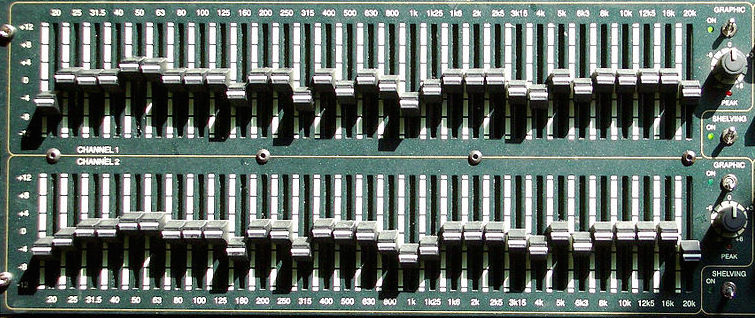
\includegraphics[width=\textwidth]{chap6/figures/faders.jpg}
	\caption{\em Each of the $r = 150$ modes can be controlled individually, analogous to a set of equalization faders. Source: Wikimedia Commons.}
\label{fig:faders}
\end{figure}

\section{Mode Coupling and Envelopes}
The simultaneous activation of all modes produces a spectrally rich timbre not dissimilar from noise. However, more refined filtering leads to a sparser spectrum, yielding a sound quality similar to musical chords. This filtering
can be achieved simply by activating only a small subset of the $r = 150$ modes at once, much as in the mode superposition study. However, such a chord is static over time, creating a dull musical effect for any prolonged 
duration. We can inject extra life into these chords by modulating their {\em envelopes}---i.e., creating time-varying amplitude envelopes around each mode. This strategy is akin to slowly adjusting the different fader knobs 
from high to low at different speeds. A simple mathematical collection of envelopes are sinusoids at different frequencies,\footnote{Oscillation: \url{https://www.youtube.com/watch?v=6nEVXFkWSZ4}} as the referenced video example illustrates. Visually, the shapes morph in and out of a slow cycle of superpositions, while the sound fades in and out of subtle frequencies of an overall chord.

\begin{figure}
	\centering
	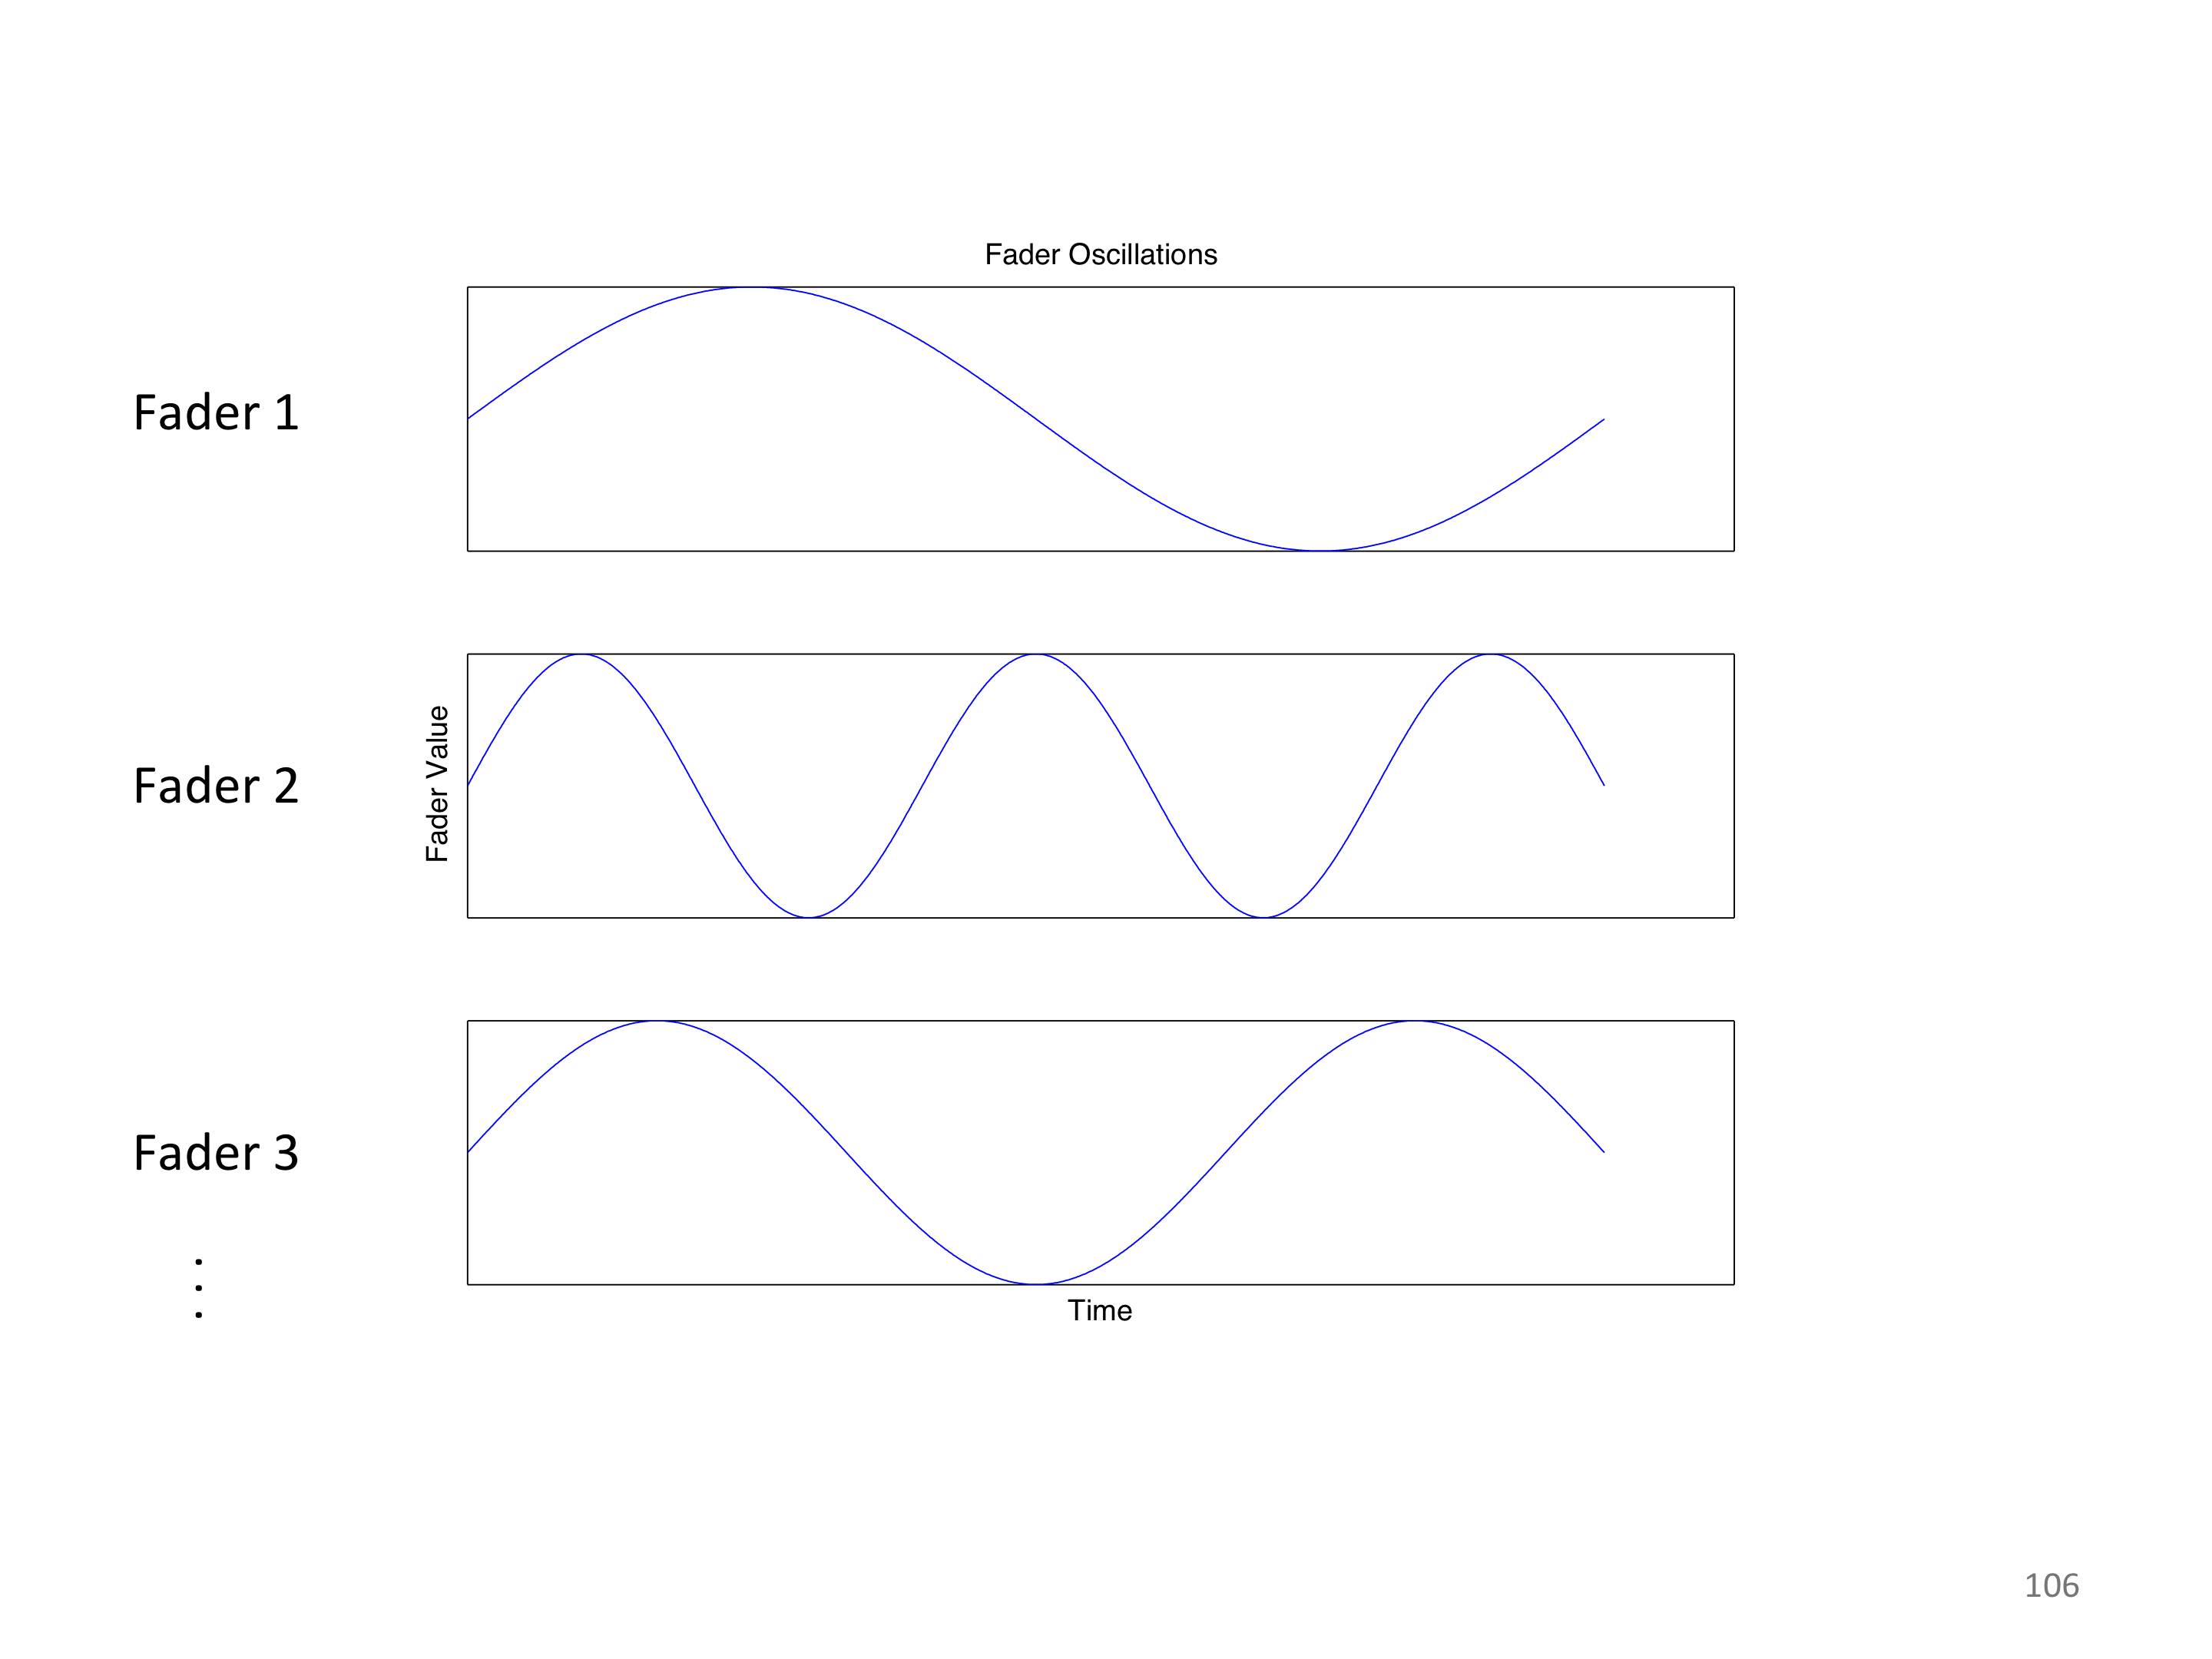
\includegraphics[width=\textwidth]{chap6/figures/fader_envelopes.png}
	\caption{\em Each modes's fader knob can be modulated smoothly over time, creating spectrally-varying envelopes.}
\label{fig:fader_envs}
\end{figure}

We can also {\em couple} different modes together, or transfer from one collection of modes smoothly into another, in analogy to a musical chord progression. As time evolves, both the amplitude envelopes and the
spectral content itself shifts, producing a complex visual and audio effect\footnote{Crossfade: \url{https://www.youtube.com/watch?v=RCIuZaWqvds}} as seen in the referenced video example.



